\chapter{Le Magnétisme Moléculaire}

\section{Définition}
Définir précisément ce qu'est un aimant moléculaire n'est pas chose aisé. Il faut bien s\^ur qu'il possède un moment magnétique non nul. Ce moment magnétique peut \^etre de spin, orbital ou bien les deux. Mais cela n'est pas suffisant. Il faut de plus, que ce moment magnétique est une orientation préférentielle. Cela se traduit par l'existence d'un axe facile, c'est à dire deux orientations qui correspondent à un minimum d'énergie pour le moment magnétique. Ces deux conditions sont les conditions minimales à remplir pour parler d'aimant moléculaire. Mais pour mettre en évidence ces propriétés, il faut qu'il soit possible de les mesurer. Autrement dit, l'anisotropie doit \^etre suffisamment forte pour que l'énergie thermique ne puisse pas retourner l'aimantation.

Cependant, l'aimant moléculaire que l'on vient de décrire n'est pas vraiment "sexy" pour reprendre les termes de Wolfgang Wernsdorfer. Ce que l'on souhaite aussi, c'est de pouvoir mettre en évidence des phénomènes quantiques tel que le retournement de l'aimantation par effet tunnel ou Quantum Tunneling of the Magnetization~(QTM) que nous décrirons plus bas. Ceci n'est possible que s'il existe, en plus de l'axe facile, un plan difficile qui permet, comme nous le verrons dans la suite, de coupler les différents états magnétique de la molécule entres eux. De plus, le spin électronique n'est pas toujours l'unique acteur du magnétisme moléculaire. Il arrive parfois que le spin nucléaire joue un r\^ole majeur dans les phénomènes quantique mesurés.

Afin de comprendre la physique associé aux aimants moléculaires, on peut donc procéder par étape. On peut tout d'abord décrire l'origine du moment magnétique non nul d'une molécule. On peut ensuite introduire la notion d'axe facile et comment elle se traduit dans le formalisme quantique. On peut ensuite aborder la notions de plan difficile, son origine et ces conséquences. Enfin, une description des interaction entre spin électronique et spin nucléaire est nécessaire pour décrire de la façon la plus complète certains aimants moléculaire, à base de lanthanide notamment.

\section{L'origine du moment magnétique}
Nous l'avons déjà dit, pour qu'une molécule puisse \^etre appelé aimant moléculaire, il faut tout d'abord qu'elle possède un moment magnétique non nul. Pour arriver à ce résulat, on peut adopter deux stratégies que je classe ici par ordre chronologique d'apparition. La première consiste à synthétiser une molécule composé de plusieurs atomes magnétique qui vont interagir entre deux pour donner un moment magnétique résultant. La deuxième technique consiste à n'utiliser un métal magnétique que l'on va venir entourer de ligands non magnétique.

\subsection{La solution a plusieurs centre}
Cette solution a été la première adopté dans le domaine du magnétisme moléculaire. Elle a permis notamment de synthéiser la désormais célèbre molécule de Mn$_{12}$-ac~(cf Fig.\ref{Mn12}). Cette dernière par exemple

\begin{figure}
\centering 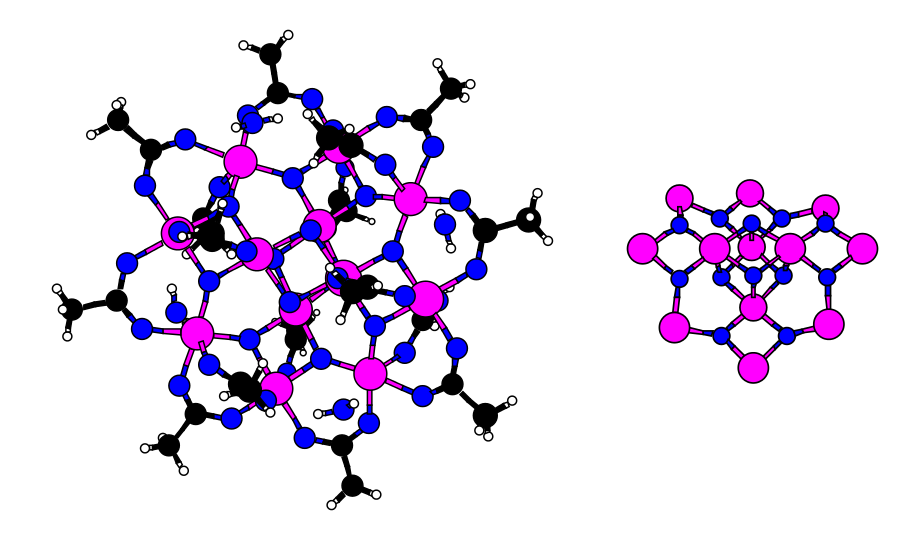
\includegraphics[scale=0.3]{Theorie/MagMol/figure1/Mn12.png} 
\caption{Sur la gauche, la molécule de Mn$_{12}$-ac. Sur la droite, le centre magnétique Mn$_{12}$O$_{12}$. Les quatre manganèses internes de spin $S=3/2$ sont antiparallèles aux huit maganèses de spin $S=2$ situés en périphérie. Le moment magnétique total résultant est $S=10$~(extrait de When Magnetism Goes Nano). Le couplage entre les différents spins est médié par les atomes d'oxygène en bleus sur la figure.}
\label{Mn12}
\end{figure}